\documentclass[journal,12pt,twocolumn]{IEEEtran}

\usepackage{setspace}
%\usepackage{gensymb}
\singlespacing
\usepackage[cmex10]{amsmath}

\usepackage{amsthm}

\usepackage{mathrsfs}
\usepackage{txfonts}
\usepackage{stfloats}
\usepackage{bm}
\usepackage{cite}
\usepackage{cases}
\usepackage{subfig}
\usepackage{float}
\usepackage{longtable}
\usepackage{multirow}

\usepackage{enumitem}
\usepackage{mathtools}
\usepackage{steinmetz}
\usepackage{tikz}
%\usepackage{circuitikz}
\usepackage{verbatim}
\usepackage{tfrupee}
\usepackage[breaklinks=true]{hyperref}
\usepackage{graphicx}
\usepackage{tkz-euclide}

\usetikzlibrary{calc,math}
\usetikzlibrary{automata, positioning}
\usepackage{listings}
    \usepackage{color}                                            %%
    \usepackage{array}                                            %%
    \usepackage{longtable}                                        %%
    \usepackage{calc}                                             %%
    \usepackage{multirow}                                         %%
    \usepackage{hhline}                                           %%
    \usepackage{ifthen}                                           %%
    \usepackage{lscape}     
\usepackage{multicol}
\usepackage{chngcntr}

\DeclareMathOperator*{\Res}{Res}

\renewcommand\thesection{\arabic{section}}
\renewcommand\thesubsection{\thesection.\arabic{subsection}}
\renewcommand\thesubsubsection{\thesubsection.\arabic{subsubsection}}

\renewcommand\thesectiondis{\arabic{section}}
\renewcommand\thesubsectiondis{\thesectiondis.\arabic{subsection}}
\renewcommand\thesubsubsectiondis{\thesubsectiondis.\arabic{subsubsection}}


\hyphenation{op-tical net-works semi-conduc-tor}
\def\inputGnumericTable{}                                 %%

\lstset{
%language=C,
frame=single, 
breaklines=true,
columns=fullflexible
}
\begin{document}


\newtheorem{theorem}{Theorem}[section]
\newtheorem{problem}{Problem}
\newtheorem{proposition}{Proposition}[section]
\newtheorem{lemma}{Lemma}[section]
\newtheorem{corollary}[theorem]{Corollary}
\newtheorem{example}{Example}[section]
\newtheorem{definition}[problem]{Definition}

\newcommand{\BEQA}{\begin{eqnarray}}
\newcommand{\EEQA}{\end{eqnarray}}
\newcommand{\define}{\stackrel{\triangle}{=}}
\bibliographystyle{IEEEtran}
\raggedbottom
\setlength{\parindent}{0pt}
\providecommand{\mbf}{\mathbf}
\providecommand{\pr}[1]{\ensuremath{\Pr\left(#1\right)}}
\providecommand{\qfunc}[1]{\ensuremath{Q\left(#1\right)}}
\providecommand{\sbrak}[1]{\ensuremath{{}\left[#1\right]}}
\providecommand{\lsbrak}[1]{\ensuremath{{}\left[#1\right.}}
\providecommand{\rsbrak}[1]{\ensuremath{{}\left.#1\right]}}
\providecommand{\brak}[1]{\ensuremath{\left(#1\right)}}
\providecommand{\lbrak}[1]{\ensuremath{\left(#1\right.}}
\providecommand{\rbrak}[1]{\ensuremath{\left.#1\right)}}
\providecommand{\cbrak}[1]{\ensuremath{\left\{#1\right\}}}
\providecommand{\lcbrak}[1]{\ensuremath{\left\{#1\right.}}
\providecommand{\rcbrak}[1]{\ensuremath{\left.#1\right\}}}
\theoremstyle{remark}
\newtheorem{rem}{Remark}
\newcommand{\sgn}{\mathop{\mathrm{sgn}}}
\providecommand{\abs}[1]{(\vert#1)\vert}
\providecommand{\res}[1]{\Res\displaylimits_{#1}} 
\providecommand{\norm}[1]{(\lVert#1)\rVert}
%\providecommand{\norm}[1]{\lVert#1\rVert}
\providecommand{\mtx}[1]{\mathbf{#1}}
\providecommand{\mean}[1]{E([ #1 )]}
\providecommand{\fourier}{\overset{\mathcal{F}}{ \rightleftharpoons}}
%\providecommand{\hilbert}{\overset{\mathcal{H}}{ \rightleftharpoons}}
\providecommand{\system}{\overset{\mathcal{H}}{ \longleftrightarrow}}
	%\newcommand{\solution}[2]{\textbf{Solution:}{#1}}
\newcommand{\solution}{\noindent \textbf{Solution: }}
\newcommand{\cosec}{\,\text{cosec}\,}
\providecommand{\dec}[2]{\ensuremath{\overset{#1}{\underset{#2}{\gtrless}}}}
\newcommand{\myvec}[1]{\ensuremath{\begin{pmatrix}#1\end{pmatrix}}}
\newcommand{\mydet}[1]{\ensuremath{\begin{vmatrix}#1\end{vmatrix}}}
\numberwithin{equation}{subsection}
\makeatletter
\@addtoreset{figure}{problem}
\makeatother
\let\StandardTheFigure\thefigure
\let\vec\mathbf
\renewcommand{\thefigure}{\theproblem}
\def\putbox#1#2#3{\makebox[0in][l]{\makebox[#1][l]{}\raisebox{\baselineskip}[0in][0in]{\raisebox{#2}[0in][0in]{#3}}}}
     \def\rightbox#1{\makebox[0in][r]{#1}}
     \def\centbox#1{\makebox[0in]{#1}}
     \def\topbox#1{\raisebox{-\baselineskip}[0in][0in]{#1}}
     \def\midbox#1{\raisebox{-0.5\baselineskip}[0in][0in]{#1}}
\vspace{3cm}
\title{Assignment 3}
\author{Taha Adeel Mohammed - CS20BTECH11052}
\maketitle
\newpage
\bigskip
\renewcommand{\thefigure}{\theenumi}
\renewcommand{\thetable}{\theenumi}
Download all python codes from 
\begin{lstlisting}
https://github.com/Taha-Adeel/AI1103/blob/main/Assignment_3/codes/assignment3.py
\end{lstlisting}
%
and latex-tikz codes from 
%
\begin{lstlisting}
https://github.com/Taha-Adeel/AI1103/tree/main/Assignment_3
\end{lstlisting}
\vspace{-3mm}
\section{Problem (GATE 2008 (CS), Q.27)}
%%(GATE 2008 (CS), Q.27) \\
Aishwarya studies either computer science or mathematics everyday. If she studies computer science on a day, then the probability she studies mathematics the next day is 0.6. If she studies mathematics on a day, then the probability she studies computer science the next day is 0.4.
Given that Aishwarya studies computer science on Monday, what is the probablity she studies computer science on Wednesday?
\begin{enumerate}[label=(\Alph*)]
\begin{multicols}{2}
%\setlength\itemsep{2em}
\item 0.24
\item 0.36
\item 0.4
\item 0.6
\end{multicols}
\end{enumerate}


\section{Solution (GATE 2008 (CS), Q.27)}
Consider the following parameters
\begin{table}[h!]
    \begin{tabular}[width=\columnwidth]{|c|m{2.4cm}|m{3.1cm}|}
         \hline
        \textbf{Parameter\hspace{-1mm}}&\textbf{Definition}&\textbf{Value}\\
        \hline    
         S&State space (i.e possible states she can be in.)& $S=\{1,2\}$, where $1$ and $2$ represents her studying CS or maths respectively on that day.\\
         \hline
         {\begin{equation*}\{X_0, X_1, \dots\}\end{equation*}}& \multicolumn{2}{p{5.8cm}|}{Random variables(which form a markov chain) where $X_i \in S$ represents her studying CS or maths on the $i$th day(i=0 for Monday)}\\
         \hline
         P& {The one \nolinebreak step state \nolinebreak transition  matrix (The elements $p_{ij}\nolinebreak=\nolinebreak\text{Pr}(X_{n+1}$ $= j\, |\, X_{n}=i)$ )}& {\vspace{-6mm}\begin{align*}
        \hspace{2em}\,\,\overbrace{
         \begin{matrix}
        1 & \,\,\,2
        \end{matrix}}^{X_{n+1}}
        \end{align*}
        \vspace{-1cm}
        \begin{align*}
        P=\scriptstyle{X_n} \bigg\{ \begin{matrix} 1\\ 2\end{matrix}
        \begin{bmatrix}
        x & \hspace{-3mm}0.6 \\
        0.4 & \hspace{-3mm}y 
        \end{bmatrix}\hspace{0.6cm}
        \end{align*}}\\
         \hline
    \end{tabular}
\end{table}


%%Consider the state space $S=\{1,2\}$, where $1$ represents Aishwarya studying CS and $2$ represents her studying maths on a particular day.\\ 
%%Let \{$X_0, X_1, \dots$ \} be a series of random variables. So we have the Markov chain  
%%\begin{align}
%%\{X_n\,|\, X_n \in S, n \geq 0\},
%%\end{align}% , where $X_n$ represents her studying CS or mathematics on the $n$th day. 
%%with initial distribution $\alpha = (\alpha_1 , \alpha_2) =(1,0)$ ($\because\alpha_i = \pr{X_0=i}$).\\
%%The state transition matrix $P=(p_{ij})$ for the markov chain (where $p_{ij}=\pr{X_{n+1}=j\, |\, X_{n}=i}$) is :-
%%\begin{align*}
%%\hspace{3.3em}\overbrace{
%% \begin{matrix}
%%1 & \,\,\,\,\,\,2
%%\end{matrix}}^{X_{n+1}}
%%\end{align*}
%%\vspace{-1cm}
%%\begin{align}
%%P\,\,=\,\,\,\,\scriptstyle{X_n\,\,} \bigg\{ \, \begin{matrix} 1\\ %%2\end{matrix}\,\,\,
%% \begin{bmatrix}
%%x & 0.6 \\
%%0.4 & y 
%%\end{bmatrix}\hspace{0.6cm}
%%\end{align}


\par As $X_n=0 \text{ and } X_n=1$ are mutually exclusive, we can easily calculate $x$ and $y$.
\begin{align}
   x=\pr{X_{n+1} = 0 |\, X_{n}=0} &= 1-\pr{X_{n+1} = 1 \,| X_{n}=0}\nonumber
    \\&= 0.4 \label{x}\\
    y=\pr{X_{n+1} = 1 |\, X_{n}=1} &= 1-\pr{X_{n+1} = 0 \,| X_{n}=1}\nonumber
    \\&= 0.6 \label{y}
\end{align}

\begin{figure}[h]
    \centering
     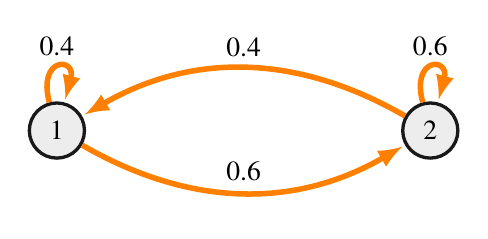
\begin{tikzpicture}[
roundnode/.style={circle, draw=black!90, fill=black!7, very thick, minimum size=7mm},
]
%Nodes
\node[roundnode]        (Computer_Science)        {1};
\node[roundnode]        (Mathematics)       [right=4cm of Computer_Science] {2};

%Lines
 \draw[every loop,
        auto=right,
        line width=0.7mm,
        >=latex,
        draw=orange,
        fill=orange]
            (Computer_Science) edge[bend right, auto=left]  node {0.6} (Mathematics)
            (Mathematics) edge[bend right, auto=right] node {0.4} (Computer_Science)
            (Computer_Science) edge[loop above]             node {0.4} (Computer_Science)
            (Mathematics) edge[loop above]             node {0.6} (Mathematics);
\end{tikzpicture}
    \par{Markov Diagram}
\end{figure}

\par The $\pr{X_{n+t}=j \,|\, X_{n}=i}$ is the $(i,j)$th position of $P^{\,t}$. Given that her initial state is $X_0=1$ ($\because$ she studies CS on Monday(n=0)).\\ Therefore $\pr{X_{2}=1 | X_{0}=1}$ ($\because$ n=2 for Wednesday) is the $(1,1)$th position of $P^2$.
\begin{align}
    P^2=\begin{bmatrix}
0.4 & 0.6 \\
0.4 & 0.6
\end{bmatrix}\times
\begin{bmatrix}
0.4 & 0.6 \\
0.4 & 0.6 
\end{bmatrix}=
\begin{bmatrix}
0.4 & 0.6 \\
0.4 & 0.6 
\end{bmatrix}
\end{align}
\par $\therefore$ The probability she studies computer science on Wednesday is $P_{1\,1}^{\,2} = 0.4$.\\
(\textbf{Ans: Option (C)})

 
%%The probability she studies CS on Wednesday($i=2$) can be found by($\because X_0=0$) :
%%\begin{align}
%%    \pr{X_2=0}&= \pr{X_1=0|X_0=0}\times \pr{X_2=0|X_1\hspace{-0.1cm}=\hspace{-0.1cm}0}\nonumber\\
%%    &+  \pr{X_1=1|X_0=0}\times \pr{X_2=0|X_1\hspace{-0.1cm}=1\hspace{-0.1cm}}\\
%%     &= 0.4\times 0.4 + 0.6\times0.4\\
%%     &=0.4
%% \end{align}
%%(\textbf{Ans: Option (C)})
\end{document}
